\chapter{La classe NP} \label{ch:capitolo11}
\subsection{Macchine di Turing non deterministiche}
Una Macchina di Turing M è una quadrupla $(Q, A, \sigma, q_0)$, dove:
\begin{itemize}
    \item Q è un insieme finito di stati
    
    \item A è un alfabeto, cui si aggiunge il simbolo bianco \#
    
    \item $\sigma$ è una funzione da Q × (A U $\{\#\}$) a p(Q × (A U $\{\#\}$) × $\{-1, +1\}$), chiamata funzione di transizione
    
    \item $q_0 \in Q$ è lo stato iniziale
\end{itemize}
Le quintuple (q, a, q', a', x ) tali che (q', a', x) $\in \sigma(q, a)$ sono dette le istruzioni di M.
\subsection{Configurazioni consecutive}
\textbf{Definizione}\\
Una configurazione istantanea di una Macchina di Turing M = (Q, A, $\sigma$, $q_0$) è un elemento dell’insieme (A U $\{\#\}$)$^*$ x Q x (A U $\{\#\}$) x (A U $\{\#\}^*$.
Nell’insieme delle configurazioni istantanee di M introduciamo la relazione binaria $\vdash_M$ che associa alla configurazione C quelle che possono seguirla in una computazione di M. Qualora non esistesse nessuna configurazione di questo tipo, scriveremo $C\vdash/_M$\\\\
\textbf{Esempio}\\
Se M ha l’istruzione (q, a, q', b, $-1$) e (q, a, q'', a, $+1$), allora.\\
\begin{figure}[htp]
    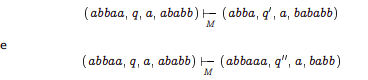
\includegraphics[scale=0.9]{tesi_stile/img/foto1cap11.png}
\end{figure}
\subsection{Computazioni}
\textbf{Definizioni}\\
\begin{itemize}
    \item La configurazione iniziale C0 di una macchina di Turing non deterministica M sull’input w è definita come nel caso deterministico,
    
    \item una sequenza
    
    $C_0\vdash_M$, $C_1\vdash_M$ ... $C_n\vdash/_M$
    
    si dirà una computazione convergente di M sull’input w.
    
    \item Diremo che M accetta w se esiste una computazione convergente di M sull’input w.
\end{itemize}
\textbf{Osservazione}\\
Quindi M accetta w se almeno una computazione di M su w converge, M rifiuta w se tutte le computazioni di M su w divergono.
\subsection{Complessità temporale per macchine di Turing non deterministiche}
\textbf{Definizione}\\
Sia M una macchina di Turing non deterministica.
Per ogni parola w accettata da M, denotiamo con $t_w$ il minimo numero di passi di una computazione convergente di M su input w.
Si dice complessità temporale di M la funzione $c_M : N \mapsto N$ definita come segue: per ogni $n \in N$
\begin{center}
    $c_M (n)$ = max$\{t_w | w accettata da M_1, l(w) <= n\}$.
\end{center}
\textbf{Osservazione}\\
Ovviamente, una macchina di Turing deterministica si può considerare come una particolare macchina di Turing non deterministica in cui, per ogni input, c’è un’unica computazione. \\
In tal caso, la definizione di $c_M (n)$ coincide con quella già data in precedenza.
\subsection{Macchine e linguaggi}
\textbf{Definizione}\\
L’insieme delle parole accettate da una macchina di Turing non deterministica M si dirà il linguaggio accettato da M.\\\\
\textbf{Proposizione}\\
I problemi accettati da macchine di Turing non deterministiche sono semi-decidibili.\\\\
\textbf{Dimostrazione}\\
Una macchina di Turing deterministica può simulare, parallelamente, le computazioni di una macchina di Turing non deterministica su un dato
input.\\
Tale macchina accetterà se almeno una delle computazioni della macchina
non deterministica termina.
\subsection{La classe NP}
\textbf{Definizione}\\
Denotiamo con NP la classe dei problemi S accettati da una macchina di Turing non deterministica M tale che $c_M(n) = O(n^k)$ per qualche intero positivo k.\\\\
\textbf{Osservazione}\\
Se $S \in NP$, allora ci sono una macchina di Turing non deterministica M, e due interi positivi c e k tali che, per ogni input w di lunghezza n, M si comporta nel modo seguente:
\begin{itemize}

    \item se $w \in S$, allora esiste almeno una computazione convergente M su w con al più c l(w) k passi
    
    \item se $w \notin S$, allora tutte le computazioni di M su w divergono.
\end{itemize}
\textbf{Osservazione}\\
Riferita ai problemi, non agli algoritmi.\\\\
\textbf{Osservazione}\\
Come quella di P, anche la definizione di NP è robusta:\\
se esiste una procedura non deterministica che accetta le parole di S e richiede l’esecuzione di $O(n^k)$ istruzioni (comunque specificate, purchè simulabili da una macchina di Turing in tempo polinomiale), allora $S \in NP$.
\subsection{SAT}
Il problema SAT è accettato dalla seguente procedura non-deterministica:\\
Dato un sitema di clausole S
\begin{enumerate}
    \item assegna (non deterministicamente) dei valori di verità alle variabili
    
    \item se tutte le clausole sono soddisfatte accetta, altrimenti divergi
\end{enumerate}
Ciascuna esecuzione del primo passo richiede tempo lineare (in termini di operazioni elementari)\\
Il secondo passo si può eseguire in tempo quadratico.
\begin{center}
    \textbf{SAT $\in$ NP}
\end{center}
\textbf{Osservazione}\\
Il passo 1 può essere eseguito in $2^k$ modi diversi, dove k è il numero delle variabili.
\subsection{3COL}
Il problema 3COL è accettato dalla seguente procedura non-deterministica:\\
Dato un grafo G
\begin{enumerate}
    \item  assegna (non deterministicamente) dei colori ai vertici
    
    \item  verifica se, per ogni lato, i vertici agli estremi hanno colore diverso
    
    \item in caso affermativo accetta, altrimenti divergi.
\end{enumerate}
Ciascuna esecuzione del primo passo richiede tempo lineare (in termini di operazioni elementari, rispetto al numero dei vertici)\\
Il secondo passo si può eseguire in tempo quadratico.
\begin{center}
    \textbf{3COL $\in$ NP}
\end{center}
\textbf{Osservazione}\\
Il passo 1 può essere eseguito in $3^k$ modi diversi, dove k è il numero dei vertici.
\subsection{Grafi}
Sia G = (V,E) un grafo e $V_0 \subseteq V$\\
L'insieme $V_0$ è indipendente se per ogni v, $v' \in V_0$, $(v, v') \notin E$.\\
L'insieme $V_0$ è una clique se per ogni v, v' $\in$ $V_0$, (v, v') $\in$ E.\\
L’insieme $V_0$ è un ricoprimento di vertici se per ogni (v, v') $\in$ E almeno uno dei vertici v,v' sta in $V_0$.\\\\
\textbf{Problema IS}\\
\textbf{Input:} Un grafo G = (V ,E) e un intero $k > 0$\\
\textbf{Output:} si se G ha un insieme\\ indipendente di ordine k, no altrimenti.\\\\
\textbf{Problema CLIQUE}\\
\textbf{Input:} Un grafo G=(V,E) e un intero $k > 0$\\
\textbf{Output:} si se G ha una clique di ordine k, no altrimenti.\\\\
\textbf{Problema VC}\\
\textbf{Input:} Un grafo G = (V,E) e un intero $k > 0$\\
\textbf{Output:} si se G ha un ricoprimento di vertici di ordine k, no altrimenti.
\subsection{Grafi-2}
\textbf{Proposizione}\\
Sia G = (V , E) un grafo e $V_0 \subseteq V$\\
Le seguenti condizioni sono equivalenti:
\begin{enumerate}
    \item $V_0$ è indipendente,
    
    \item $V_0$ è una clique del grafo complementare $\Bar{G} = (V , \Bar{E})$
    
    \item V / $V_0$ è un ricoprimento di vertici.
\end{enumerate}
\textbf{Corollario}\\
Ognuno dei problemi IS, CLIQUE e VC si riduce agli altri due.\\
Inoltre la funzione di riduzione si calcola rapidamente.\\\\
\textbf{Dimostrazione}\\
Sia G un grafo di ordine n. Allora.\\
\begin{figure}[htp]
    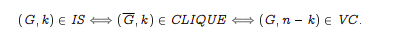
\includegraphics[scale=0.9]{tesi_stile/img/foto2cap11.png}
\end{figure}\\
\textbf{Osservazione}\\
I sottoinsiemi di V di ordine k sono 
$
\begin{pmatrix}
& n & \\
& k &
\end{pmatrix}	
$
e quindi non polinomialmente limitati da n (se k non è fissato).
\subsection{Grafi-3}
Il problema IS è accettato dalla seguente procedura non-deterministica:\\
Dato un grafo G e un intero $k > 0$.
\begin{enumerate}
    \item seleziona (non deterministicamente) k vertici
    
    \item verifica se, per ogni coppia di vertici selezionati v, v', (v, v') $\notin$ E
    
    \item in caso affermativo accetta, altrimenti divergi.
\end{enumerate}
Ciascuna esecuzione del primo passo richiede tempo polinomiale (in termini di operazioni elementari, rispetto al numero dei vertici) come pure il secondo passo.\\
In maniera simile, si trovano procedure non-deterministiche che accettano CLIQUE e VC, con la medesima complessità:
\begin{center}
    \textbf{IS, CLIQUE, VC $\in$ NP}
\end{center}
\subsection{coNP}
\textbf{Definizione}\\
coNP è la classe dei problemi il cui complemento sta nella classe NP.\\\\
\textbf{Osservazione}\\
Mentre P = coP, non è noto se NP = coNP.\\\\
\textbf{Proposizione}\\
$P \subseteq NP \cap coNP$
\subsection{Un'altra definizione di Np}
\textbf{Proposizione}\\
Sia $S \subseteq A^*$ un problema. Le seguenti condizioni sono equivalenti
\begin{enumerate}
    \item Esistono una macchina di Turing non deterministica M e un intero $k > 0$ tali che M accetta S e $c_M (n) = O(n^k)$
    
    \item Esistono un problema $T \subseteq A^* x B^*$ e un polinomio p(n) tali che $T \in P$ e per ogni $w \in A^*$
\end{enumerate}
\begin{figure}[htp]
    \centering
    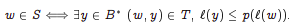
\includegraphics[scale=0.9]{tesi_stile/img/foto3cap11.png}
\end{figure}
\textbf{Osservazione}\\
In altri termini, ogni problema di classe NP  sull’alfabeto A si ottiene da un sottoinsieme di classe P di $A^* x B^*$ con le due operazioni seguenti:
\begin{enumerate}
    \item Si scartano le coppie (w, y) con y' molto più lungo di w
    
    \item si proietta su $A^*$
\end{enumerate}
Sia S un problema che verifica la condizione 2\\
Per ogni $w \in S$, ci sarà una parola y tale che $(w, y) \in T$ e $l(y) <= p(l(w)$).\\
Chiameremo y il testimone (o soluzione) di w.\\
\newpage
\subsection{Il testimone}
Sia S un problema che verifica la condizione 2.\\
Per ogni $w \in S$, ci sarà una parola y tale che (w, y) $\in$ T e l(y)$ <= $p(l(w)).
Chiameremo y il testimone (o soluzione) di w.\\\\
\textbf{Osservazione}\\
La limitazione l(y)$ <= $ p(l(w)) serve ad assicurare che la condizione
(w, y) $\in$ T possa essere accertata in tempo polinomiale rispetto a l(w).
Invero, T è accettato da una macchina di Turing deterministica M tale che
$c_M(n) <= q_1(n)$, per un opportuno polinomio a coefficienti non negativi $q_1$.
Sia $q_2(n) = q_1(n + (p(n)))$. Se
\begin{center}
   (w, y) $\in$ T, l(y) $<=$ p(l(w)),
\end{center}
Allora M converge su (w, y) in al più $q_1(l(w) + l(y)) <= q_2(l(w)$) passi.\\\\
\textbf{Esempi}
\begin{figure}[htp]
    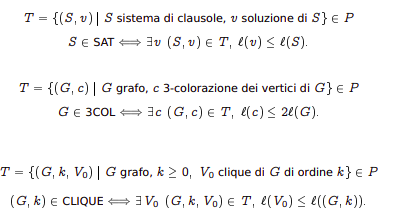
\includegraphics[scale=0.9]{tesi_stile/img/foto4cap11.png}
\end{figure}
\newpage
\subsection{Dimostrazione}
\begin{figure}[htp]
    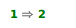
\includegraphics[scale=0.9]{tesi_stile/img/foto5cap11.png}
\end{figure}
Esistono una macchina di Turing non deterministica M e un polinomio q(n) tali che M accetta S e $c_M (n) <= q(n)$.\\
Poniamo p(n) = q(n)(n + q(n) + 2).\\
Ogni $w \in S$ ha una computazione convergente con non più di q(l(w)) passi.\\
Tale computazione è descritta da una parola di lunghezza al più p(l(w)).\\
Poniamo\\
\begin{center}
    \item T = \{(w, y) | y computazione convergente di M su input w\}
\end{center}
Si ha $T \in P$ e\\
\begin{figure}[htp]
    \centering
    
\includegraphics[scale=0.9]{tesi_stile/img/foto6cap11.png}
\end{figure}
\begin{figure}[htp]
    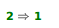
\includegraphics[scale=0.9]{tesi_stile/img/foto7cap11.png}
\end{figure}\\
Esistono un problema $T \in P$ e un polinomio p(n) tali che
\begin{figure}[htp]
    \centering
    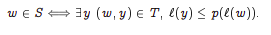
\includegraphics[scale=0.9]{tesi_stile/img/foto10cap11.png}
\end{figure}
Il problema S è accettato dalla seguente procedura non-deterministica:\\
Dato w
\begin{enumerate}
    \item genera (non deterministicamente) y tale che $l(y)<= p(l(w))$
    
    \item verifica se (w, y) $\in$ T
    
    \item in caso affermativo accetta, altrimenti divergi
\end{enumerate}
Ciascuna esecuzione del primo passo richiede tempo polinomiale rispetto alla lunghezza di w.\\
L’esecuzione del secondo passo richiede tempo polinomiale rispetto alla
lunghezza di (w, y), che è maggiorata da $l(w) + p(l(w))$.\\
Quindi l’esecuzione del secondo passo richiede tempo polinomiale rispetto
alla lunghezza di w.





